
%(BEGIN_QUESTION)
% Copyright 2007, Tony R. Kuphaldt, released under the Creative Commons Attribution License (v 1.0)
% This means you may do almost anything with this work of mine, so long as you give me proper credit

This water filter level control system uses an ultrasonic level transmitter to sense the level of water in the filter, and a controller to drive a motor-actuated valve introducing raw water to be filtered:

$$\includegraphics[width=15.5cm]{i02370x01.eps}$$

Assuming a direct-acting level transmitter (increasing filter level = increasing signal), and a signal-to-open control valve (increasing controller output signal = wider open valve), determine whether the level controller needs to be configured for {\it direct-action} or {\it reverse-action}, and explain your reasoning.  Annotate the diagram with ``+'' and ``$-$'' symbols next to the PV and SP controller inputs to show more explicitly the relationships between the controller inputs and output.

\vskip 10pt

Next, determine the response of the controller to the following situations.  In other words, determine what the controller's output signal will do when this water level control system is affected in the following ways:

\begin{itemize}
\item{} A sudden increase in effluent flow rate (clean water demand)
\vskip 10pt 
\item{} Level transmitter fails high (indicating 100\% full water level)
\vskip 10pt 
\item{} Control valve actuator fails, driving valve fully open (ignoring controller signal)
\vskip 10pt 
\medskip

\vskip 20pt \vbox{\hrule \hbox{\strut \vrule{} {\bf Suggestions for Socratic discussion} \vrule} \hrule}

\begin{itemize}
\item{} Re-draw the diagram for this water filter level control system, replacing the controller (circle) with an op-amp symbol (triangle), determining the ``+'' and ``$-$'' input assignments on the opamp for PV and SP.
\item{} Explain why level control is important in a water filter such as this.
\item{} What do the ``H'' and ``L'' symbols near the LIR represent?
\end{itemize}

\underbar{file i02370}
%(END_QUESTION)





%(BEGIN_ANSWER)

This controller needs to be {\it reverse-acting}:

$$\includegraphics[width=15.5cm]{i02370x02.eps}$$

This re-drawing of the control system uses an opamp symbol in place of the ISA-standard circle used to represent a loop controller:

$$\includegraphics[width=15.5cm]{i02370x03.eps}$$

\begin{itemize}
\item{} A sudden increase in effluent flow rate (clean water demand): {\it controller output increases}
\vskip 10pt 
\item{} Level transmitter fails high (indicating 100\% full water level): {\it controller output decreases}
\vskip 10pt 
\item{} Control valve actuator fails, driving valve fully open (ignoring controller signal): {\it controller output decreases}
\vskip 10pt 
\medskip


%(END_ANSWER)





%(BEGIN_NOTES)








\vskip 20pt \vbox{\hrule \hbox{\strut \vrule{} {\bf Virtual Troubleshooting} \vrule} \hrule}

This question is a good candidate for a ``Virtual Troubleshooting'' exercise.  Presenting the diagram to students, you first imagine in your own mind a particular fault in the system.  Then, you present one or more symptoms of that fault (something noticeable by an operator or other user of the system).  Students then propose various diagnostic tests to perform on this system to identify the nature and location of the fault, as though they were technicians trying to troubleshoot the problem.  Your job is to tell them what the result(s) would be for each of the proposed diagnostic tests, documenting those results where all the students can see.

During and after the exercise, it is good to ask students follow-up questions such as:

\begin{itemize}
\item{} What does the result of the last diagnostic test tell you about the fault?
\item{} Suppose the results of the last diagnostic test were different.  What then would that result tell you about the fault?
\item{} Is the last diagnostic test the best one we could do?
\item{} What would be the ideal order of tests, to diagnose the problem in as few steps as possible?
\end{itemize}












\vfil \eject

\noindent
{\bf Summary Quiz:}

$$\includegraphics[width=15.5cm]{i02370x01.eps}$$

Suppose someone dumps a bunch of soap in the water headed for the filtration plant, resulting in a thin but dense layer of foamy bubbles floating on top of the water.  The ultrasonic level transmitter, which uses sound waves to measure distance, senses this foam.  What effect will this have on the actual water level in the filter over time, due to the control system's action?

\begin{itemize}
\item{} There will be no ill effect -- the liquid level will be right on setpoint
\vskip 5pt 
\item{} The actual liquid level will be a bit more than it should
\vskip 5pt 
\item{} The actual liquid level will oscillate above and below setpoint
\vskip 5pt 
\item{} The water filter will run completely dry (no liquid)
\vskip 5pt 
\item{} The actual liquid level will be a bit less than it should
\vskip 5pt 
\item{} The water filter will completely overflow with liquid
\end{itemize}



%INDEX% Basics, control loop troubleshooting: determining cause of control problem
%INDEX% Process: water filter level control

%(END_NOTES)


